%!TEX root = ../../architekturdokumentation.tex
\chapter{Prozesse und Threads}
	\section{Datenbank}
	Die SQL Server Datenbank garantiert die ACID Prinzipien. Sämtliche Datenzugriffe sollen in Transaktionen erfolgen, damit die Integrität der Datenbank sicherstellt.
	
	\subsection{Optimistic Concurrency}
	Jede Eingabemaske von VoluntaryO soll für das Handling von Concurrency Problemen das Verfahren Optimistic Concurrency einsetzen. Dies bedeutet, dass man Concurrency Konflikte erlaubt, dann aber korrekt darauf reagiert.
	Das Entity Framework erlaubt einem das Erkennen von solchen Konflikten über das Werfen von OptimisticConcurrencyExceptions. Dafür muss die Datenbank und das Datenmodell aber korrekt konfiguriert sein.
	Möglich macht dies das Einfügen einer Tracking-Column, die angibt wann eine Spalte das letzte mal geändert wurde. Dann kann Entity Framework so konfiguriert werden, dass diese Column in jedem SQL-Update- oder Delete-Command über die Where-Clausel abgefragt wird. Wenn keine Felder upgedatet werden, interpretiert EF dies automatisch al Concurrency-Konflikt.
	
	\section{Server}
	\begin{wrapfigure}[8]{R}{0.5\textwidth}
  		\vspace{-25pt}
	  	\begin{center}
    		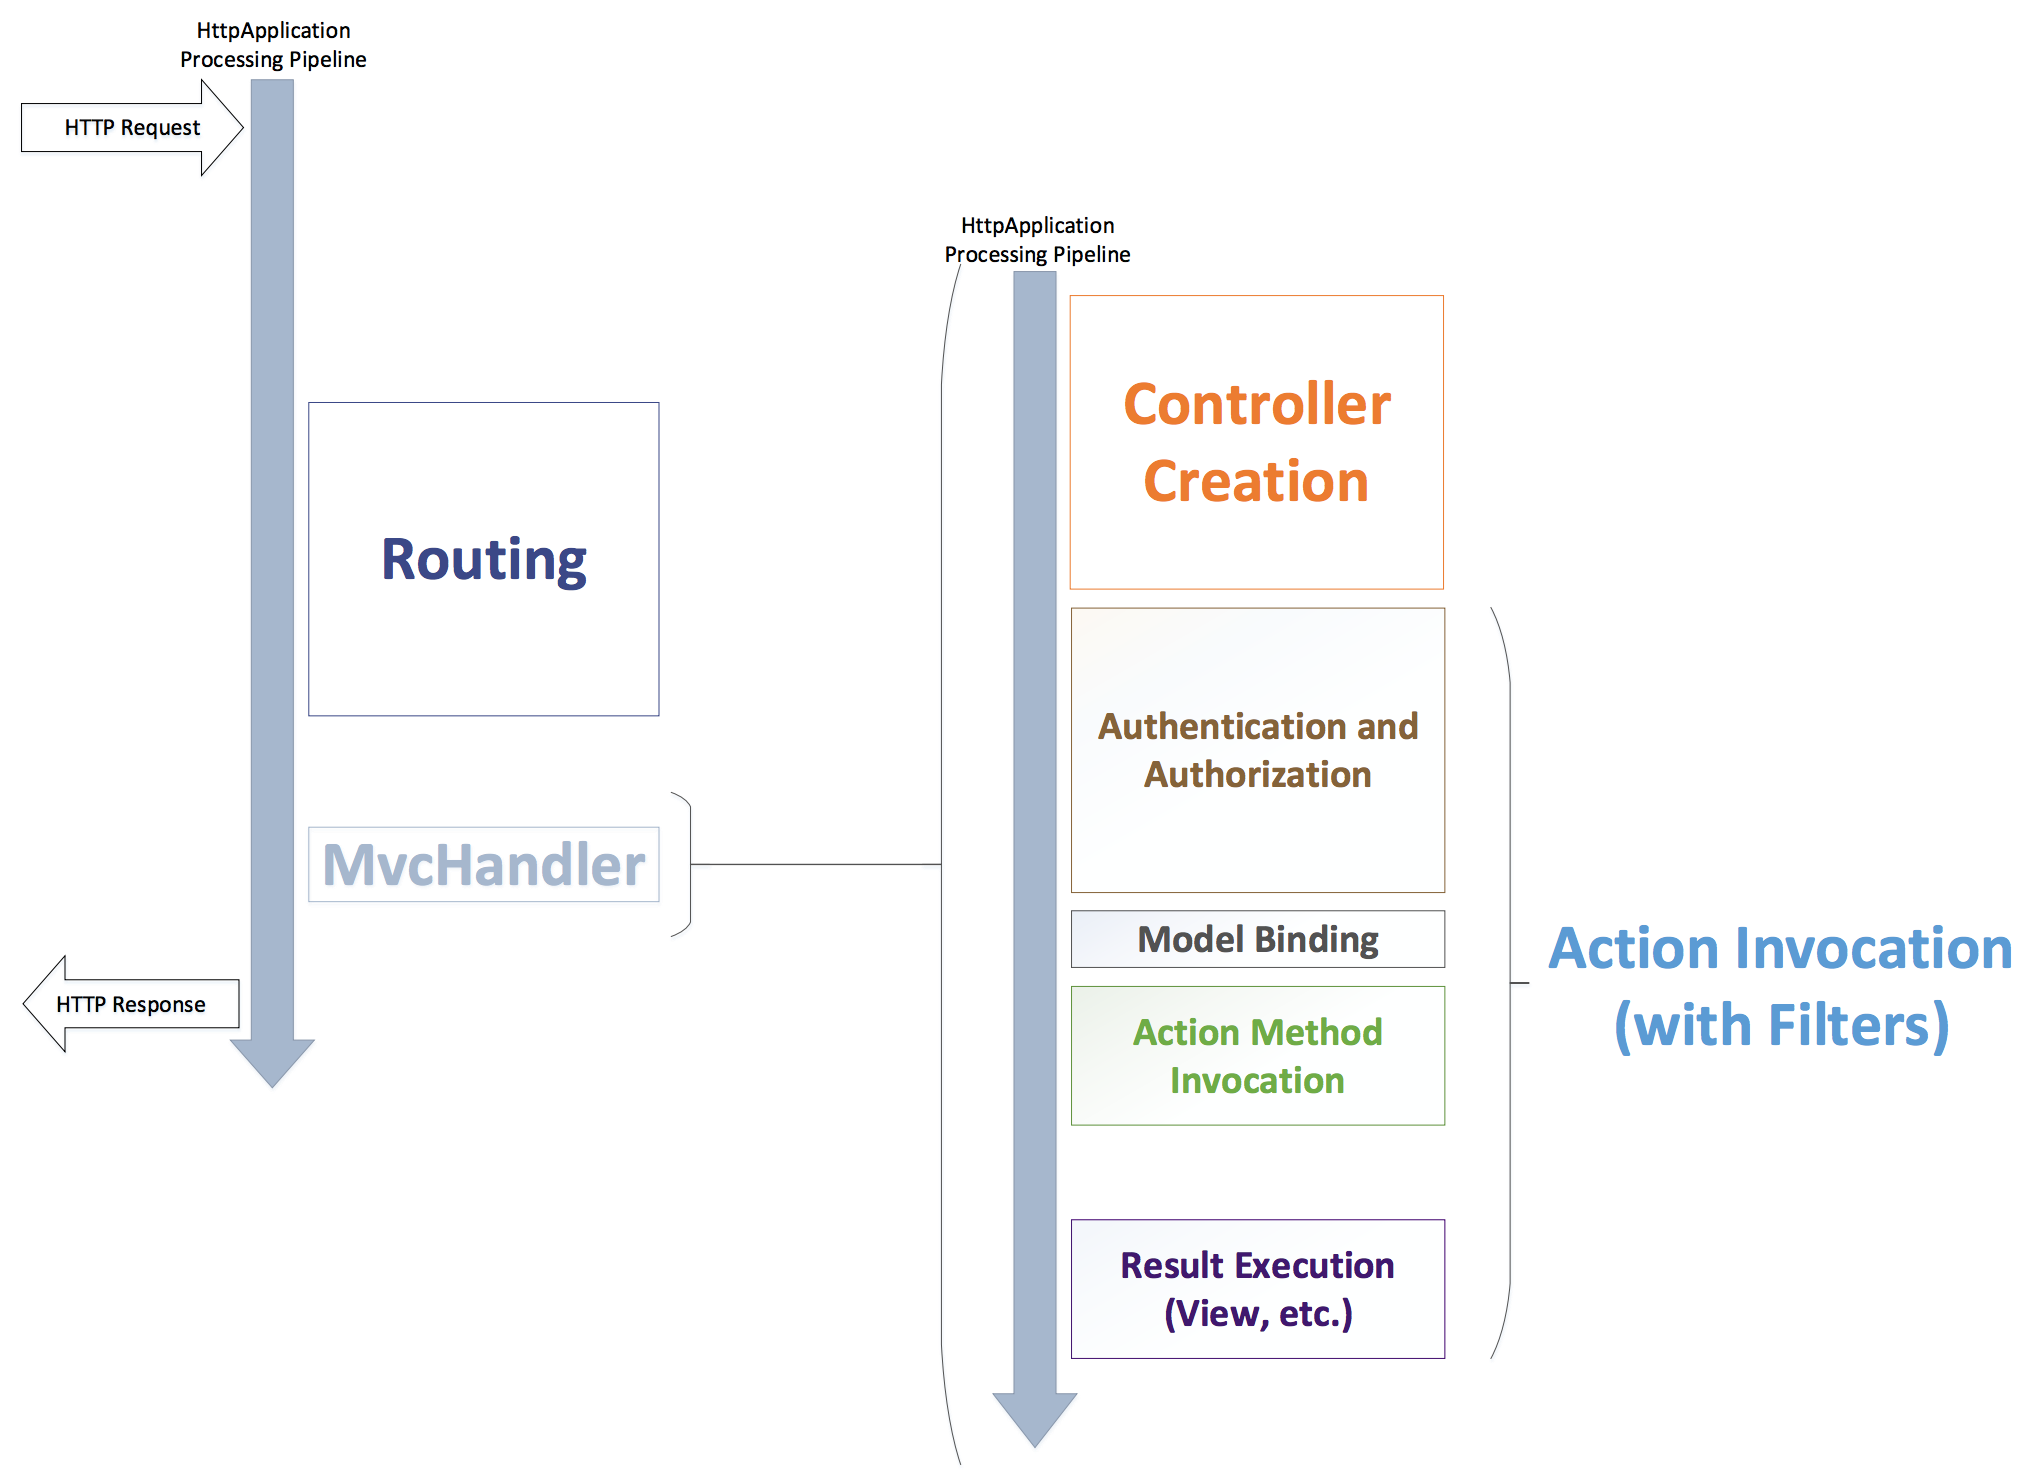
\includegraphics[height=7cm]{content/architekturdokumentation/images/ApplicationLifecycle.png}
	  	\end{center}
  		\vspace{-20pt}
	 	\caption{Application Lifecycle eines Requests}
	\end{wrapfigure}
	Die Requests, also die Controller, werden untereinander nicht synchronisiert. Für jeden Request werden neue Instanzen der Objekte erstellt. Somit können Race-Conditions auf Objektbasis vermieden werden. Die Zugriffe auf die Persistenzebene werden durch Transaktionen geschützt.
	
	